% 
% Annual Cognitive Science Conference
% Sample LaTeX Two-Page Summar -- Proceedings Format
% 

% Original : Ashwin Ram (ashwin@cc.gatech.edu)       04/01/1994
% Modified : Johanna Moore (jmoore@cs.pitt.edu)      03/17/1995
% Modified : David Noelle (noelle@ucsd.edu)          03/15/1996
% Modified : Pat Langley (langley@cs.stanford.edu)   01/26/1997
% Latex2e corrections by Ramin Charles Nakisa        01/28/1997 
% Modified : Tina Eliassi-Rad (eliassi@cs.wisc.edu)  01/31/1998
% Modified : Trisha Yannuzzi (trisha@ircs.upenn.edu) 12/28/1999 (in process)
% Modified : Mary Ellen Foster (M.E.Foster@ed.ac.uk) 12/11/2000
% Modified : Ken Forbus                              01/23/2004
% Modified : Eli M. Silk (esilk@pitt.edu)            05/24/2005
% Modified : Niels Taatgen (taatgen@cmu.edu)         10/24/2006
% Modified : David Noelle (dnoelle@ucmerced.edu)     11/19/2014
% Modified : Roger Levy (rplevy@mit.edu)     12/31/2018

%% Change "letterpaper" in the following line to "a4paper" if you must.

\documentclass[10pt,letterpaper]{article}

\usepackage{cogsci}
\usepackage{graphicx}
\usepackage{xcolor}

%\cogscifinalcopy % Uncomment this line for the final submission 
\twopagesummarysubmission % switch for two-page summary submissions so
                          % that they're never anonymized 


\usepackage{pslatex}
\usepackage{apacite}
\usepackage{float} % Roger Levy added this and changed figure/table
                   % placement to [H] for conformity to Word template,
                   % though floating tables and figures to top is
                   % still generally recommended!

\usepackage[none]{hyphenat} % Sometimes it can be useful to turn off
%hyphenation for purposes such as spell checking of the resulting
%PDF.  Uncomment this block to turn off hyphenation.




%\setlength\titlebox{4.5cm}
% You can expand the titlebox if you need extra space
% to show all the authors. Please do not make the titlebox
% smaller than 4.5cm (the original size).
%%If you do, we reserve the right to require you to change it back in
%%the camera-ready version, which could interfere with the timely
%%appearance of your paper in the Proceedings.



\title{Convolutional Neural Networks Can (Meta-)Learn the Same-Different Relation}
 
\author{
    {\large \bf Max Gupta}$^1$,
    {\large \bf Sunayana Rane}$^1$,
    {\large \bf R. Thomas McCoy}$^2$,
    {\large \bf Thomas L. Griffiths}$^{1,3}$ \\ 
    \texttt{mg7411@princeton.edu, srane@princeton.edu, tom.mccoy@yale.edu, tomg@princeton.edu} \\
    $^1$Department of Computer Science, Princeton University \\
    $^2$Department of Linguistics and Wu Tsai Institute, Yale University \\
    $^3$Department of Psychology, Princeton University
}


\begin{document}

\newcommand{\mccoy}[1]{\textcolor{blue}{\textbf{McCoy: #1}}}
\newcommand{\griffiths}[1]{\textcolor{red}{\textbf{Griffiths: #1}}}

\maketitle



\begin{abstract}
While convolutional neural networks (CNNs) have come to match and exceed human performance in many visual reasoning tasks, the tasks these models optimize for are largely constrained to the level of individual objects, such as classification and captioning. Humans remain vastly superior to CNNs in visual tasks involving relations, including the simple, cognitively foundational ability to identify two objects as `same' or `different'. A number of studies have shown that while CNNs can be coaxed into learning the same-different relation in some settings, they tend to generalize poorly to other instances of this relation. In this work we show that the same CNN architectures that fail to generalize the same-different relation with conventional training are able to succeed when trained via meta-learning, which explicitly encourages abstraction and generalization across tasks.   

\end{abstract}

\begin{quote}
\small
\textbf{Keywords:} 
Meta-Learning; Relational Reasoning; Similarity
\end{quote}

\section{Introduction}

Debates about what aspects of human learning can be captured by artificial neural networks have played a prominent role in the history of cognitive science \cite{minsky1969introduction, rumelhart1986learning, pinker1988language, fodor1988connectionism}. One recent manifestation of this question has focused on the learning capacities of convolutional neural networks (CNNs), which are widely used in computer vision and have been used to capture aspects of human behavioral and neural responses in object recognition tasks \cite{kubilius2019brain, peterson2018evaluating}. Despite strong performance capturing the features of objects, these models seem to fall short when learning about relations between objects. 

The human capacity for abstraction is based on  understanding the laws that govern relations. The most basic of these abilities, arguably a precursor to more complex abstract reasoning, is the same-different relation: the ability to tell if two objects are the same or not. Extensive work in cognitive science dating back to the 1980's \cite{premack1983codes} has shown that this ability develops early on in human childhood \cite{blote1999young}, is associated with the learning of language \cite{lupker2015there}, and extends far and wide in the animal kingdom, from bees to ducklings and chimpanzees \cite{gentner2021learning}. However, learning the same-different relation has proven surprisingly difficult for artificial neural networks. Early convolutional neural networks were shown to have difficulty on the same-different task in \citeA{kim2018not}. Subsequent work has suggested that CNNs can learn some forms of the same-different relation given a well-structured training regime and near-distribution testing regime \cite{puebla2022can, geiger2020relational}, though they still struggle with true out-of-distribution generalization. These results have led to the tentative conclusion that CNNs may lack the inductive biases needed to learn abstract relational information. 

\begin{figure}[htb!]
    \centering
    \includegraphics[width=\columnwidth]{figures/fig1.png}
    \caption{Example of a same-different task as it is posed to a convolutional neural network (CNN) at test-time. Given an image containing two objects, the CNN should return a label of 1 if the two objects are the same or a label of 0 if they are different (as in the example input to the left of the figure)}
    \label{fig:cnn}
\end{figure}

These negative results do not mean that neural networks are incapable of representing the same-different relation. As models have become larger and more advanced, we have very recently begun to see generalizable understanding of same-different relations emerging in state of the art vision-transformer models pre-trained on ImageNet with methods such as contrastive learning \cite{dosovitskiy2020image, tartaglini2023deep}. The observation that some very large neural networks are able to learn this relation motivates re-investigating  whether shallower CNNs have the capacity to learn the relation. 

Previous attempts to train CNNs on the same-different relation have used standard techniques for training neural networks, in which a task (or set of tasks) is defined and the weights of the network are optimized to perform that task (or set of tasks). Recently, researchers have begun to explore a different technique for training neural networks, known as meta-learning \cite<e.g.,>[]{finn2017model}. Using this technique, a set of neural networks are each trained to perform a different task, and the shared initial weights of those neural networks are optimized to increase the performance of all networks across all tasks. The learned initial weights encode
%abstract away 
the shared structure of the different tasks, making it easier for the individual networks to learn to perform those tasks. Meta-learning has been shown to allow simple neural networks to quickly learn to perform tasks that previously were assumed to require symbolic representations, such as learning formal languages \cite<e.g.,>[]{mccoy2023modeling}. In this paper, we explore whether this tendency to find generalizable abstractions is sufficient to allow CNNs to learn the same-different relation.

%The inductive biases of a learning system include all of the factors, other than the data, that determine what that system learns. Existing investigations of the ability of CNNs to learn the same-different relation have focused on one aspect of inductive bias: the architecture of these neural networks. Focusing on this distinctive architecture is reasonable: inspired by biological visual systems, it incorporates convolutions that result in translation invariance. This is a strong form of inductive bias and is partly responsible for the popularity of CNNs in computer vision, as it results in weights being shared across the visual field and hence reduces the amount of data that these systems need to learn the values of those weights. However, architecture is not the only source of inductive biases. Artificial neural networks trained by gradient descent are biased towards functions that can be expressed by weights that are close to the weights used to initialize learning. Those initial weights thus constitute another potential source of inductive bias. In this paper, we use meta-learning as a training mechanism to reach a weight pattern that facilitates strong generalizable performance on same-different relations, demonstrating that CNNs can learn these abstract relations when trained with a different learning algorithm.

%; indeed, methods outside of architecture design, such as training paradigms and loss functions, may be equally likely to introduce helpful inductive biases into a deep learning system. In this study, we demonstrate how meta-learning can introduce an inductive bias that allows CNNs to reliably learn the elusive same-different relation.

\section{Background}

\subsection{Convolutional neural networks}

Convolutional neural networks are a type of multi-layered artificial neural network that takes pixel-level visual data as input \cite{lecun2015deep}. Key components of the CNN architecture take  inspiration from biological visual processing systems \cite{hubel1959receptive}. The initial layers of the network learn filters that are applied across an image, with their outputs being spatially pooled to form representations that are translation invariant and expressed at different scales. The learned filters have been shown to detect features, such as edges, which are useful for tasks such as image classification. Modern CNNs use architectural advancements such as residual layers \cite<the resulting models are called ResNets;>[]{he2016deep} to train deeply layered models on a variety of tasks. CNNs first came to prominence for their remarkable image classification ability \cite{krizhevsky2012imagenet}, and have since matched or surpassed human performance on a variety of visual tasks \cite{alzubaidi2021review}. As such, CNNs are often used as models for human visual processing. 

\subsection{Learning the same-different relation}

Various forms of CNNs have been trained and tested on relational visual tasks. A common dataset used for training and evaluation is the Synthetic Visual Reasoning Test (SVRT) dataset, a battery of 23 different visual-relation tasks \cite{fleuret2011comparing}. In early experiments, CNN architectures that were very successful in image classification tasks were largely unsuccessful on the visual-relation tasks in the SVRT dataset \cite{stabinger201625}. The underlying reason for this gap was not well understood. However, it was clear that CNNs were not achieving human-level performance on abstract visual relation tasks in the same way that they were on image classification tasks. It remained an open question whether this was because CNNs lack the human-like inductive biases necessary for visual reasoning. 

As CNN architectures improved and showed heightened performance on computer vision problems, further studies investigated whether these more sophisticated architectures were able to solve visual relation tasks such as same-different. A study using a CNN architecture with increased multi-layered attention mechanisms, for example, showed that the more sophisticated architecture significantly improved performance on a range of relational classification tasks \cite{wang2016relation}. This suggested that, under certain circumstances, forms of the CNN architecture might be capable of achieving strong performance on relational tasks. However, further studies on same-different tasks in particular yielded mixed results. A recent study investigated various CNN architectures on same-different tasks and found that while the networks could perform well on same-different tasks that were similar to the tasks in their training data, their performance dropped significantly when tested on another family of same-different tasks that were substantially different from those in the training data (although the abstract visual relation tested was, of course, the same) \cite{puebla2022can}. This outcome was also true for larger, deeper, more sophisticated CNN architectures such as ResNets, leading to the conclusion that abstract same-different relations were difficult or impossible for CNNs to learn in a generalizable manner. 

\subsection{Meta-learning}
While previous work has suggested that these  results indicate that CNNs may not have the architectural inductive biases needed to robustly learn abstract visual relations such as same-different, another source of  relevant inductive biases is the training paradigm that is used. All evaluations of CNNs in previous work have learned a set of weights by training models to perform a single task or set of tasks simultaneously. In this paper we use a different approach: meta-learning. In particular, we focus on the Model-Agnostic Meta-Learning (MAML) algorithm \cite{finn2017model}, which is designed to find the optimal starting point in weight space for a set of related tasks, such that the model can rapidly generalize to new, unseen tasks. 

%One hypothesis from the cognitive science literature is that children learn to learn the same-different relation through repeated exposure to many different stimuli across varied environments in which  comparisons are readily available. 

Given a set of tasks ${\cal T}$ such that each task $t \in {\cal T}$ has an associated loss function ${L}_t$, conventional neural network training seeks a set of weights for a neural network  $\phi$ that minimizes the loss function 
\begin{equation}
{\cal L}_{\rm \, conventional} = \sum_{t \in {\cal T}} { L}_t (\phi) 
\end{equation}
which is simply the sum of the losses across different tasks. By contrast, MAML seeks to find the initial weights $\theta$ that minimize the loss function
\begin{equation}
{\cal L}_{\rm \, MAML} = \sum_{t \in {\cal T}} { L}_t ( \phi_t) \qquad {\rm for} \ \phi_t = \theta - \alpha \nabla { L}_t(\theta) 
\end{equation}
where $\phi_t$ are a set of weights adapted for performing task $t$ via gradient descent applied to the loss $L_t$ of task $t$ starting at the initial weights $\theta$ (with $\alpha$ being a learning rate). The resulting $\theta$ should capture the regularities shared by the tasks in ${\cal T}$, supporting abstraction and generalization (see Figure~\ref{fig:metaexplanatory}).

%This training technique, which many in the machine learning and cognitive science community have dubbed 'metalearning' has become widely successful in few-shot learning (citations), human developmental modeling (citations), language acquisition (citations, McCoy Griffiths), and numerous other areas of cognitive science. 

In this work, we explore whether meta-learning allows convolutional neural networks to form generalizable representations of the same-different relation, challenging previous accounts suggesting certain neural architectures lack the capacity to capture same-different reasoning 
%is outside the scope of certain neural architectures 
\cite{kim2018not, puebla2022can}. We replicate previous studies testing CNNs of varying depths and switch the conventional training regime to one based on meta-learning, looking for the emergence of a reliable generalization of same-different understanding across novel stimuli and in novel tasks. Importantly, the networks that we train are exposed to exactly the same training data regardless of whether the networks are optimized using conventional training or meta-learning; the only difference is the type of optimization algorithm that is applied to the data. Matching the data allows us to isolate the effect of this algorithm. %(conventional learning vs.\ meta-learning).


\begin{figure}[t]
    \centering
    %\figuretitle{}
    \includegraphics[width=\columnwidth]{figures/SDmetafig.png}
    \caption{Meta-learning initial weights for generalization. A neural network with a standard initialization ($\theta$) typically requires a large amount of training to learn a specific task. Meta-learning optimizes the network's initialization to create a meta-learned initialization $\theta^*$ from which a range of different tasks can be learned with a small amount of training. In our setting, we use meta-learning not for its typical purpose of enabling the rapid learning of many tasks but rather as a way to encourage abstraction.}
    \label{fig:metaexplanatory}
\end{figure}



\section{Replicating Previous Work}

Throughout all experiments, we replicate the same CNN architectures evaluated by \citeA{kim2018not}, who tested performance on the SVRT dataset for CNNs of varying depths and convolutional filter sizes (exact hyper-parameters specified in the original paper copied in Appendix A). In addition to the original Problem 1 from the SVRT challenge (pictured in Figure~\ref{fig:cnn}) we also train on 9 same-different tasks created by \citeA{puebla2022can}, which augment the standard SVRT dataset with new shapes such as arrows, irregular polygons, and shapes with random colors (the full set is shown in Figure~\ref{fig:augmented}). In the standard learning setting, same-different tasks are processed as individual input/label pairs: an image and a corresponding 0/1 label for different/same (Figure ~\ref{fig:cnn} illustrates this at test-time, where the label is withheld). Note that, in these datasets, what constitutes a distinct "task" is a particular type of shape over which same-different judgments must be made. For instance, one task is based on irregular polygons while another is based on regular polygons. Thus, all tasks target the same abstract relation (same-different), but they instantiate this relation with different types of shapes. An example of a full episode as presented to the models is shown in Appendix B (add episode visual)


\begin{figure*}[bt]
    \centering
    \includegraphics[width=\linewidth]{figures/pb_examples_grid.pdf}
    \caption{The Same-Different dataset from Puebla and Bowers (2022). Each column shows one of the nine tasks in this dataset, where all tasks are based around the same-different relation but use different types of shapes to instantiate that relation. Each task has a stochastic function generator that ensures each example is unique within any given dataset. }
    \label{fig:augmented}
\end{figure*}


To establish a baseline, we first evaluate the performance of three CNN architectures in this setting, training each model end-to-end on all 10 distinct tasks, with equal frequency for each task and for the categories of \textit{same} and \textit{different}. We test the CNN architectures used by Kim et al. with 2, 4, and 6 convolutional layers using max pooling, batch normalization, and ReLU activation, followed by 3 fully connected layers of 1024 units each and a 2-dimensional classification layer. All models are trained with Adam optimization \cite{kingma2015adam} and a base learning rate of 1e-3. 

We then test each model on unseen same-different examples from the 10 tasks the model has been trained on, as a basic in-distribution test of learning these tasks. Averaging over 10 seeds run to convergence, we find performance stabilizing almost exactly at the level of random guessing for all three model depths (Figure~\ref{fig:fig4}, left); since there are two possible labels (\textit{same} and \textit{different}), random guessing would yield an accuracy of 50\%. As an exception to this general trend, some conditions do manage to reliably converge to high-accuracy solutions (in particular, a 2-layer CNN achieves 99 percent test-time accuracy on the scrambled task and 80 percent accuracy on the lines task). A potential explanation is that the scrambled and lines tasks are the only tasks in the dataset that just feature straight, right-angled lines, a low-level feature that develops earlier in shallower networks but may be overlooked in deeper networks. 

\begin{figure*}[bt]
    \centering
    \includegraphics[width=0.9\textwidth]{figures/metabaseline.pdf}
    \caption{In-distribution same-different classification accuracy for a vanilla-learner (left) versus a meta-learner (right) by task and architecture. The vanilla learner is trained using standard gradient descent, while the meta-learner is trained with the algorithm MAML in a way that is intended to encourage abstraction. Each bar is one version of the same-different task, where the task versions differ in terms of what types of shapes are used to illustrate same-different relations. These evaluations are in-distribution because the models' training data always contained examples of the same type being evaluated on. "Original" represents task \#1 from the SVRT dataset. Error bars represent standard deviations from mean accuracy across 10 randomly initialized seeds.}
    \label{fig:fig4}
\end{figure*}



\section{Meta-learning Same-Different In-Distribution}

Having established the performance of a class of CNNs on the augmented same-different dataset, we move to formalizing the meta-learning setup of the task. Without changing the model architecture or the content or quantity of data, we change the learning algorithm from standard stochastic gradient descent to MAML in order to explore the impact of using meta-learning.  

In the meta-learning setting, we generate 'episodes' from each of 
%the previously seen tasks 
task
consisting of labeled support sets for task-specific adaptation and query sets with held-out labels for evaluation. The meta-learner then has a chance to 'practice' on the episode's support set before outputting predictions for each query image. Crucially, each episode contains examples from exactly one task. Within-episode learning constitutes the 'inner loop' of standard learning from the support set -- the gradient step taken from the initial weights $\theta$ -- for which we provide a 'fast' inner learning rate of 1e-2. To aid the model in learning from a diversity of episode structures, we use variable support set sizes of evenly distributed same/different examples (4, 6, 8, and 10 examples) and fixed query sizes (3 examples, always). 


The outer loop consists of the transfer of learning across task-specific episodes and is associated with the more gradual transfer of knowledge from one task to other tasks, for which we assign a 'slower' learning rate of 1e-4 and use Adam optimization. Following standard methodology, we add a validation stage to monitor model performance on unseen episodes from the same task-set. 

By using this outer-loop update which optimizes for generalization across examples, we intend to create pressure for the learner to go beyond example-specific properties toward a more generalizable notion of sameness/difference (see Discussion). This generality is further encouraged by sampling episodes alternating across task types and support sizes.
%By sampling episodes alternating across task types and support sizes, we create pressure for the learner to go beyond task or episode specific properties, towards a more generalizable notion of sameness/difference.
We ensure that our meta-learning models (described in this section) and our vanilla models (described in the previous section) receive exactly the same training data as follows: We first generate the dataset for the meta-learning setting as described in the previous paragraphs, sampling a support set and a query set for each of the 1000 episodes that we produce for each of the 10 tasks. The training data used for the vanilla models in the previous section are then created by 'flattening' this meta-learning dataset -- that is, the vanilla training set is the concatenation of all support sets and all query sets from all episodes in the meta-learning training set. 

As a first step, we test the three previously described CNN architectures in our meta-learning setup by meta-training on 1000 episodes from each of the 10 tasks and testing on unseen episodes from the same tasks. A 2-layer CNN performs at chance on the majority of tasks seen in-distribution, but we see a striking increase in performance as we increase convolutional depth (Figure~\ref{fig:fig4}, right). A CNN with 6 convolutional layers performs at almost perfect accuracy across all tasks it has been meta-trained on, and its accuracy is consistent across seeds.\footnote{For full results, see Appendix A}
%and represents more certainty in the distribution of its predictions 
This suggests that these deeper networks are better able to respond to the pressure for abstraction that we intend to create via meta-learning.
%capture and learn from the enhanced diversity presented during meta-training. 
The bias-variance tradeoff formalizes this observation: deeper networks have more tunable parameters, resulting in less bias and an increased ability to represent variance in the dataset. However, if a neural network can perform well on data sampled in-distribution (as shown here), one possible explanation is that the network has simply learned to memorize shallow properties of its data distribution, and not to generalize the abstract notion of sameness and difference---a concern that motivates the analyses in the next section.


\section{Meta-learning Same-Different Out-of-Distribution: Leave-One-Out}

In this section, we aim to further investigate the ability of meta-trained CNNs to capture a generalizable notion of sameness/difference by testing on unseen, out-of-distribution tasks. To set this up, we perform a leave-one-out test, training the previously highest performing model (the 6-layer CNN) on the same battery of same-different classification problems, but crucially holding out one task from training for testing. In this way, we systematically test the model on out-of-distribution tasks it has never seen during training. We do this for all tasks and meta-train to convergence with MAML, using the same parameters described above. 

The results are shown in Figure~\ref{fig:fig5}. 
We intentionally replicate the structure of this experiment from \citeA{puebla2022can}, who found that even much larger, pre-trained ResNet architectures were unable to reliably generalize out-of-distribution on this set of tasks using standard learning techniques. By using this setup in a meta-learning context, we see that even much shallower CNNs without pre-training can reliably generalize to even the most challenging OOD tasks.  

\begin{figure*}[htb!]
    \centering
    \includegraphics[width=0.9\textwidth]{figures/metaood.png}
    \caption{Out-of-distribution same-different classification accuracy for a CNN trained using meta-learning. Each bar shows one version of the same-different task, where the versions differ in terms of the types of shapes used to illustrate same-different relations. A separate CNN was meta-trained for each bar, where the meta-training process included all tasks except the one to be evaluated on, and then evaluated on that withheld task. Thus, the task being evaluated on was always out-of-distribution.}
    \label{fig:fig5}
\end{figure*}

Classification accuracies were at or about 95 percent in all tasks except for three (arrows, lines, and scrambled). These three tasks were also found to be hardest for ResNets in the analysis performed by \citeA{puebla2022can}. In our case, however, meta-learning allows even these shallower CNNs to outperform ResNets in each of these 'failure' cases by significant margins, and with much less data. For example in the worst performing task ('lines'), previous results showed ResNet50 and ResNet152 performing at chance accuracy, whereas we show a meta-trained CNN consistently performs above chance (where chance level is 50\%).\footnote{Although \citeA{puebla2022can} did not release exact details on data quantity during training, ImageNet pretraining allows the models to see over 1 million images prior to fine-tuning on the same-different task.}

\section{Naturalistic Experiments}

While the data from Puebla and Bowers consists of   stochastically generated, simplistic shapes we would like to be able to verify the performance and behavior of these models on image data from the real world. To this end, we conducted a series of experiments testing the above suite of convolutional neural networks on same-different pairings of real world objects from Brady et al. (add citation). Surprisingly, we demonstrate similarly strong generalization trends hold across the board when meta-learning from this naturalistic data. First as a more stringent test of generalization, we load the model weights trained on data from Puebla and Bowers, measuring a far out-of-distribution generalization ability to the significantly more pixel-dense, challenging naturalistic stimuli of the type shown in Figure X (add figure). Second, we train the same set of models end to end on the naturalistiic data from Brady et al. holding out unseen examples for testing. 


\section{Weight Space Analysis}

What are the internal representations the model is learning? Where is the same-different relation embedded / learned in the weights? 

\section{Discussion}

By using a training algorithm based on meta-learning, we have shown that CNNs can successfully learn the same-different relation even though they struggle to do so when they are trained with more standard optimization approaches.
%By reformulating the same-different task as a meta-learning problem, we have seen that convolutional neural networks can learn to overcome architectural limitations in relational reasoning ability. 
CNNs trained via meta-learning can perform same-different classification with high accuracy (exceeding 95\% in most conditions) even when the input is based on types of images that never appeared in the meta-training data, indicating that these networks have internalized a version of same-different relations that is abstract enough to generalize to new types of shapes.
While much work has recently focused on novel  architectures dedicated to improving relational reasoning in vision models \cite{webb2021emergent,kerg2022inductive,altabaa2024abstractors,webb2024relational}, our results demonstrate that an alternative pathway toward enhanced relational reasoning is via the nature of the training algorithm: optimizing a standard CNN (without architectural modifications) using meta-learning rather than standard learning. 
%training regime that more explicitly prioritizes training diversity and abstraction can provide an alternative pathway to abstract relational reasoning. (sentence about PIP, Irie, Lake). 

What is it about meta-learning that leads to the enhanced same-different reasoning we have observed? One possible explanation is that it may provide an incentive for abstraction. To understand this point, it is useful to compare meta-learning to standard learning. In standard learning, a network is shown a batch of examples, and its weights are then adjusted such that, if it were to process those same examples again, it would achieve a smaller error on them. 
%Thus, weight updates are made based on one set of examples with the goal of improving performance on the same set of examples. 
In contrast, in meta-learning, each batch of examples (i.e., each episode) has two parts: the support set and the query set. A copy of the network is trained on the support set and evaluated on the query set, and the original network's weights are then adjusted such that, if it were trained again on the support set, its performance on the query set would improve.
Thus, meta-learning incentivizes the model to be able to learn from one set of examples (the support set) in a way that is useful for processing a different set of examples (the query set).
This pressure for generalizing from one set of examples to another might facilitate abstraction because low-level features (e.g., the angles of particular shapes) are unlikely to be broadly useful, whereas more abstract features (e.g., same-different information) will have more general utility.

%In some ways, t
These results add to a growing body of evidence that meta-learning can enable neural networks to overcome some of their most notorious limitations \cite{irie2024neural}. For instance, meta-learning can increase neural network abilities in few-shot learning \cite{hochreiter2001learning,mccoy2023modeling}, compositionality \cite{lake2023human}, and out-of-distribution generalization \cite{finn2017model}. 
However, the nature of the advantage that meta-learning provides is different in our work than in previous work. 
Traditionally, meta-learning serves as a targeted weight-initialization method: %involves exposing the network to many different tasks (with each meta-learning episode instantiating a different task), and 
it is used to identify a starting point from which a network can efficiently learn many different tasks. This starting point encodes inductive biases that have been acquired through the meta-learning process and that enable the network to subsequently learn and generalize more effectively.
In contrast, our use of meta-learning functions more as a training algorithm than as a weight initialization algorithm. Rather than having a network meta-learn from episodes that each instantiate a different task, we have networks meta-learn from episodes that all instantiate the same task (same-different classification) but with variation in the types of inputs that are used. Therefore, rather than instilling the ability to learn many different tasks (as is more typical in meta-learning), our usage modifies the way in which the network learns a single task. Specifically, as argued in the previous paragraph, the goal in our usage of meta-learning is to optimize for cross-example generalization in a way that facilitates abstraction. Our results suggest that the approach has indeed had this effect.




%increase training diversity and practice can instantiate an inductive bias towards relational reasoning in vanilla CNN's. 
%\textcolor{red}{meta-learning puts a natural pressure/provides an incentive towards abstraction... (TODO)} I gave this a shot above! - TM

%\section{Conclusion}

To a large extent, modern computer vision has advanced through optimizing 
%Modern deep learning, especially computer vision, has proven successful largely through optimizing
classification objectives for individual objects, where objects are recognized by the statistical pattern generated by their individual pixels. 
What can be left out in the process is the rich 'invisible' space between objects that humans seem to make sense of effortlessly: how individual objects relate to one another. By using meta-learning to train a neural network on same-different tasks, this work provides a path to imbue stronger pressures
%priors 
for neural networks to reason relationally across novel stimuli, using the higher-order nature of the gradient updates in meta-learning to encourage the development of more abstract relational information inside neural networks.

\section{Acknowledgments}
MG acknowledges support from the Princeton AI Teaching Fellowship. 
%{insert ack's here}
We also gratefully acknowledge the computational resources provided by the Della high-performance computing cluster at Princeton University, which were essential for meta-training the models presented in this study. This work was supported by grant N00014-23-1-2510 from the Office of Naval Research.

% Place acknowledgments (including funding information) in a section at
% the end of the paper.

\nocite{ChalnickBillman1988a}
\nocite{Feigenbaum1963a}
\nocite{Hill1983a}
\nocite{OhlssonLangley1985a}
% \nocite{Lewis1978a}
\nocite{Matlock2001}
\nocite{NewellSimon1972a}
\nocite{ShragerLangley1990a}

%\clearpage

\bibliographystyle{apacite}

\setlength{\bibleftmargin}{.125in}
\setlength{\bibindent}{-\bibleftmargin}

\bibliography{CogSci_Template}

% ===== APPENDIX SECTION START =====
% This section should be placed after your main content but before \end{document}

% Start on a new page and begin appendix
\clearpage
\appendix

% Title for the appendix section
\section{Appendix A}
\label{app:detailed_results}

% Single wide table with both results side by side
\begin{table}[h!]
\centering
\resizebox{\textwidth}{!}{%
\begin{tabular}{|l|c|c|c||c|c|c|}
\hline
& \multicolumn{3}{c||}{\textbf{Vanilla Learning (Acc \%)}} & \multicolumn{3}{c|}{\textbf{Meta-Learning (Acc \%)}} \\
\hline
\textbf{Task} & \textbf{2-Layer} & \textbf{4-Layer} & \textbf{6-Layer} & \textbf{2-Layer} & \textbf{4-Layer} & \textbf{6-Layer} \\
\hline
regular & $50.0 \pm 0.0$ & $50.0 \pm 0.0$ & $50.0 \pm 0.0$ & $52.2 \pm 5.0$ & $85.8 \pm 9.9$ & $98.5 \pm 0.7$ \\
lines & $79.5 \pm 24.1$ & $50.0 \pm 0.0$ & $50.0 \pm 0.0$ & $78.6 \pm 8.0$ & $94.8 \pm 14.9$ & $100.0 \pm 0.1$ \\
open & $51.4 \pm 4.3$ & $50.0 \pm 0.0$ & $50.0 \pm 0.0$ & $48.8 \pm 6.0$ & $85.2 \pm 10.3$ & $97.5 \pm 0.8$ \\
wider\_line & $50.0 \pm 0.0$ & $50.0 \pm 0.0$ & $50.0 \pm 0.0$ & $52.2 \pm 5.0$ & $84.2 \pm 10.4$ & $97.8 \pm 0.7$ \\
scrambled & $99.1 \pm 0.6$ & $50.0 \pm 0.0$ & $50.0 \pm 0.0$ & $82.0 \pm 7.0$ & $94.4 \pm 14.8$ & $99.9 \pm 0.1$ \\
random\_color & $55.0 \pm 0.0$ & $55.0 \pm 0.0$ & $55.0 \pm 0.0$ & $49.8 \pm 4.0$ & $86.3 \pm 7.2$ & $95.0 \pm 0.7$ \\
arrows & $50.0 \pm 0.0$ & $50.0 \pm 0.0$ & $50.0 \pm 0.0$ & $48.6 \pm 6.0$ & $69.0 \pm 11.6$ & $93.5 \pm 1.8$ \\
irregular & $50.0 \pm 0.0$ & $54.2 \pm 12.5$ & $50.0 \pm 0.0$ & $45.4 \pm 5.0$ & $83.0 \pm 12.3$ & $99.2 \pm 0.4$ \\
filled & $52.4 \pm 7.2$ & $50.0 \pm 0.0$ & $50.0 \pm 0.0$ & $54.0 \pm 6.0$ & $84.2 \pm 13.4$ & $97.9 \pm 0.6$ \\
original & $50.0 \pm 0.0$ & $50.0 \pm 0.0$ & $50.0 \pm 0.0$ & $51.0 \pm 5.0$ & $84.0 \pm 10.9$ & $97.0 \pm 1.3$ \\
\hline
\textbf{Average} & $58.7 \pm 16.0$ & $50.9 \pm 1.7$ & $50.5 \pm 1.6$ & $56.3 \pm 12.6$ & $85.1 \pm 7.2$ & $97.6 \pm 2.0$ \\
\hline
\end{tabular}}
\end{table}

\begin{center}
\parbox{\textwidth}{
\centering
\large\textbf{Table 1: Performance comparison between vanilla learning and meta-learning approaches}\\[0.3em]
\normalsize Results show mean accuracy (\%) ± standard deviation over 10 random seeds for each CNN architecture on the tasks from \cite{puebla2022can}. Chance performance is 50\%.
}
\end{center}


\clearpage

\section{Appendix B: Episode Visualizations}

\begin{figure}[H]
    \centering
    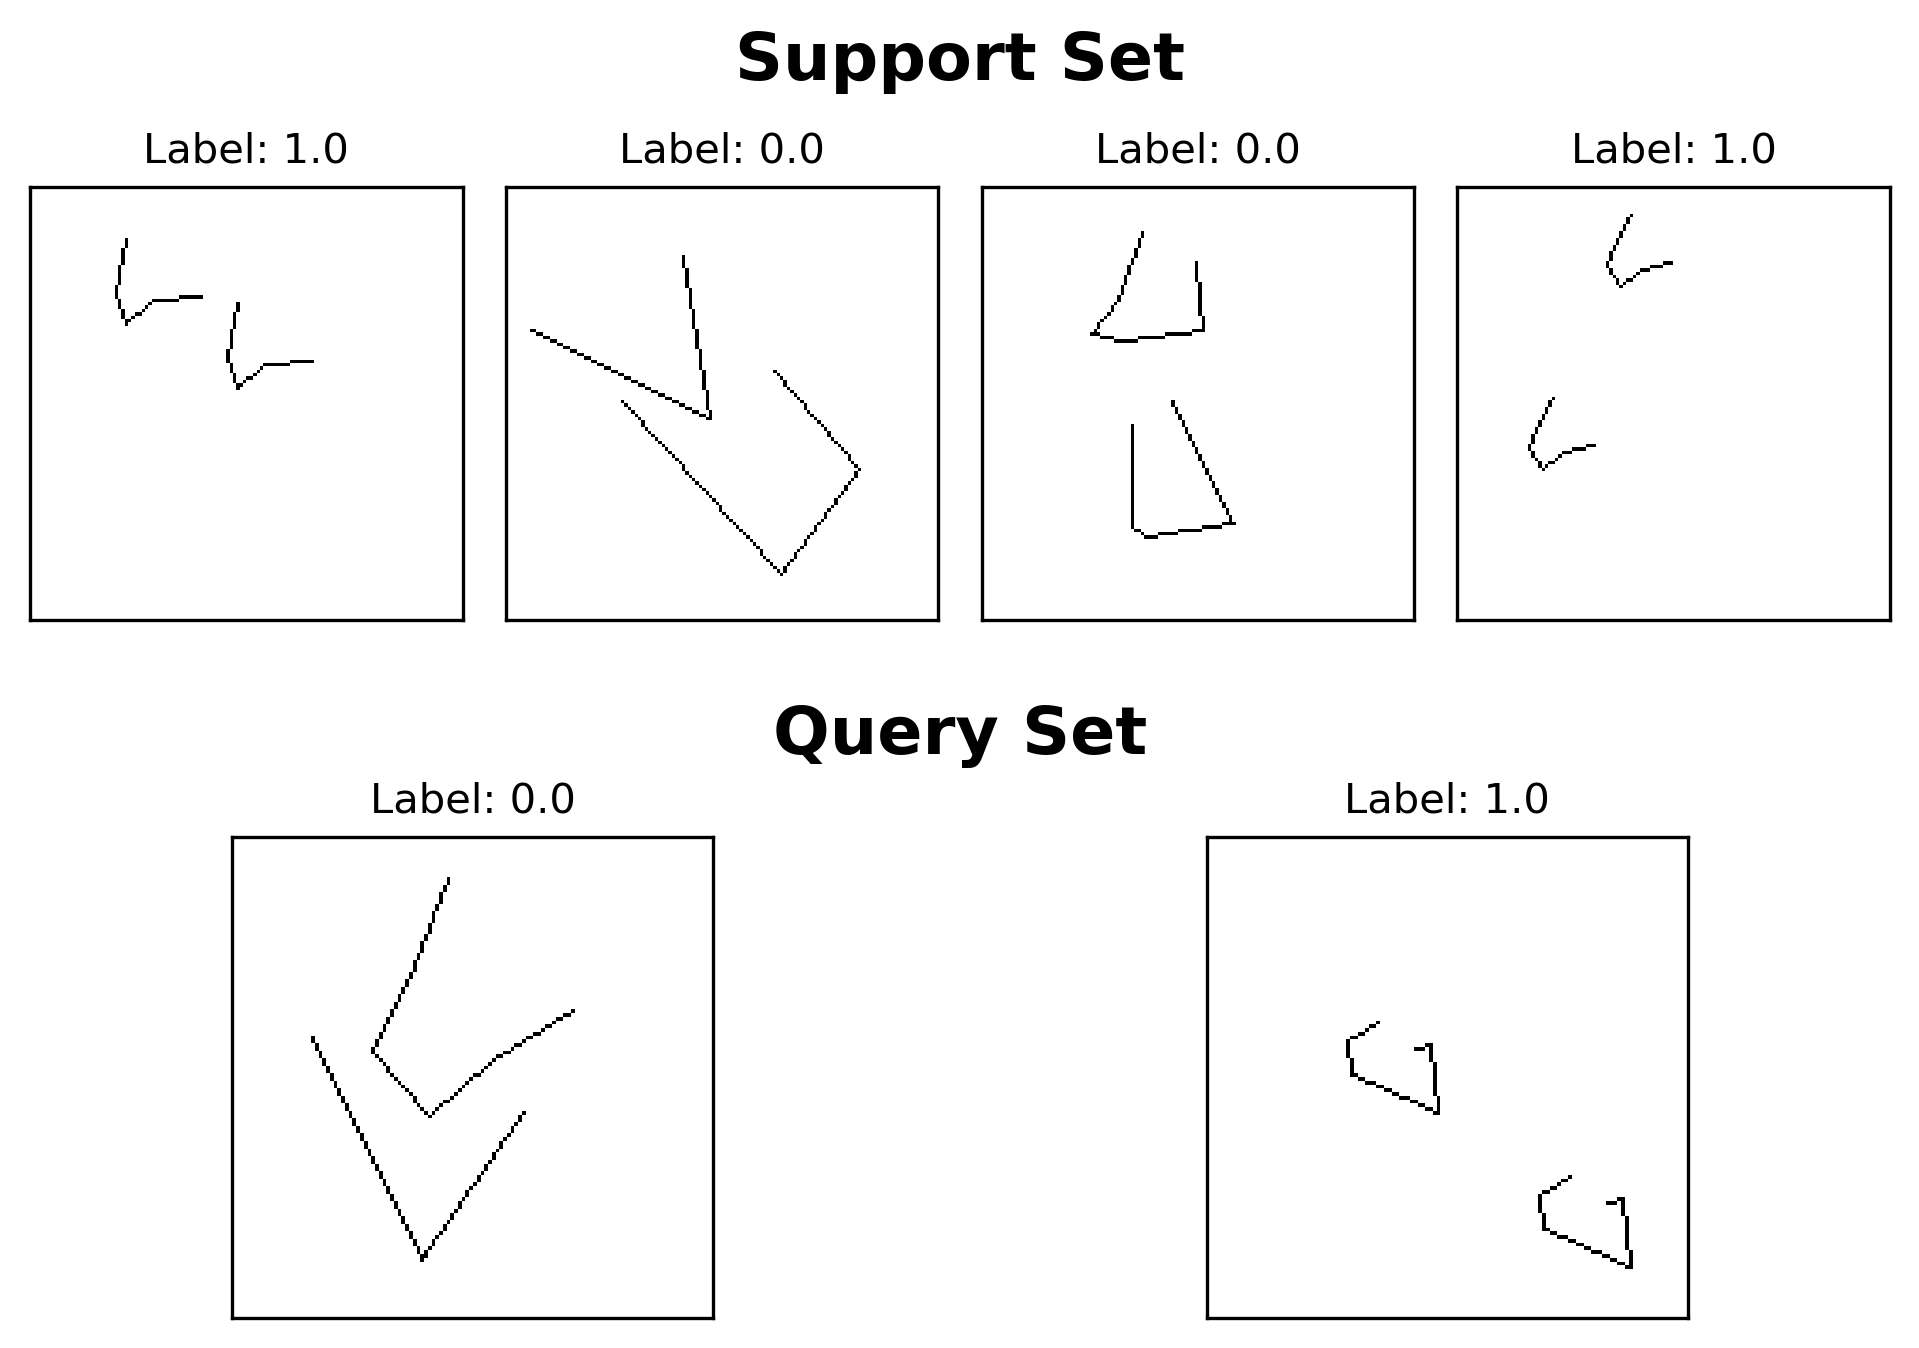
\includegraphics[width=0.9\columnwidth]{figures/open_support4_ep0_boxed.png}
    \caption{A single episode of the 'open' task from Puebla and Bowers (2022) as presented to the model at training and test time. Note: this particular example has support set size of 4 example and a query set size of 2 examples, but we randomly intermix support set sizes to promote better generalization at test time and to prevent the model from simply memorizing the statistics of its training episodes. 
    }
    \label{fig:open_episode}
\end{figure}

\begin{figure}[H]
    \centering
    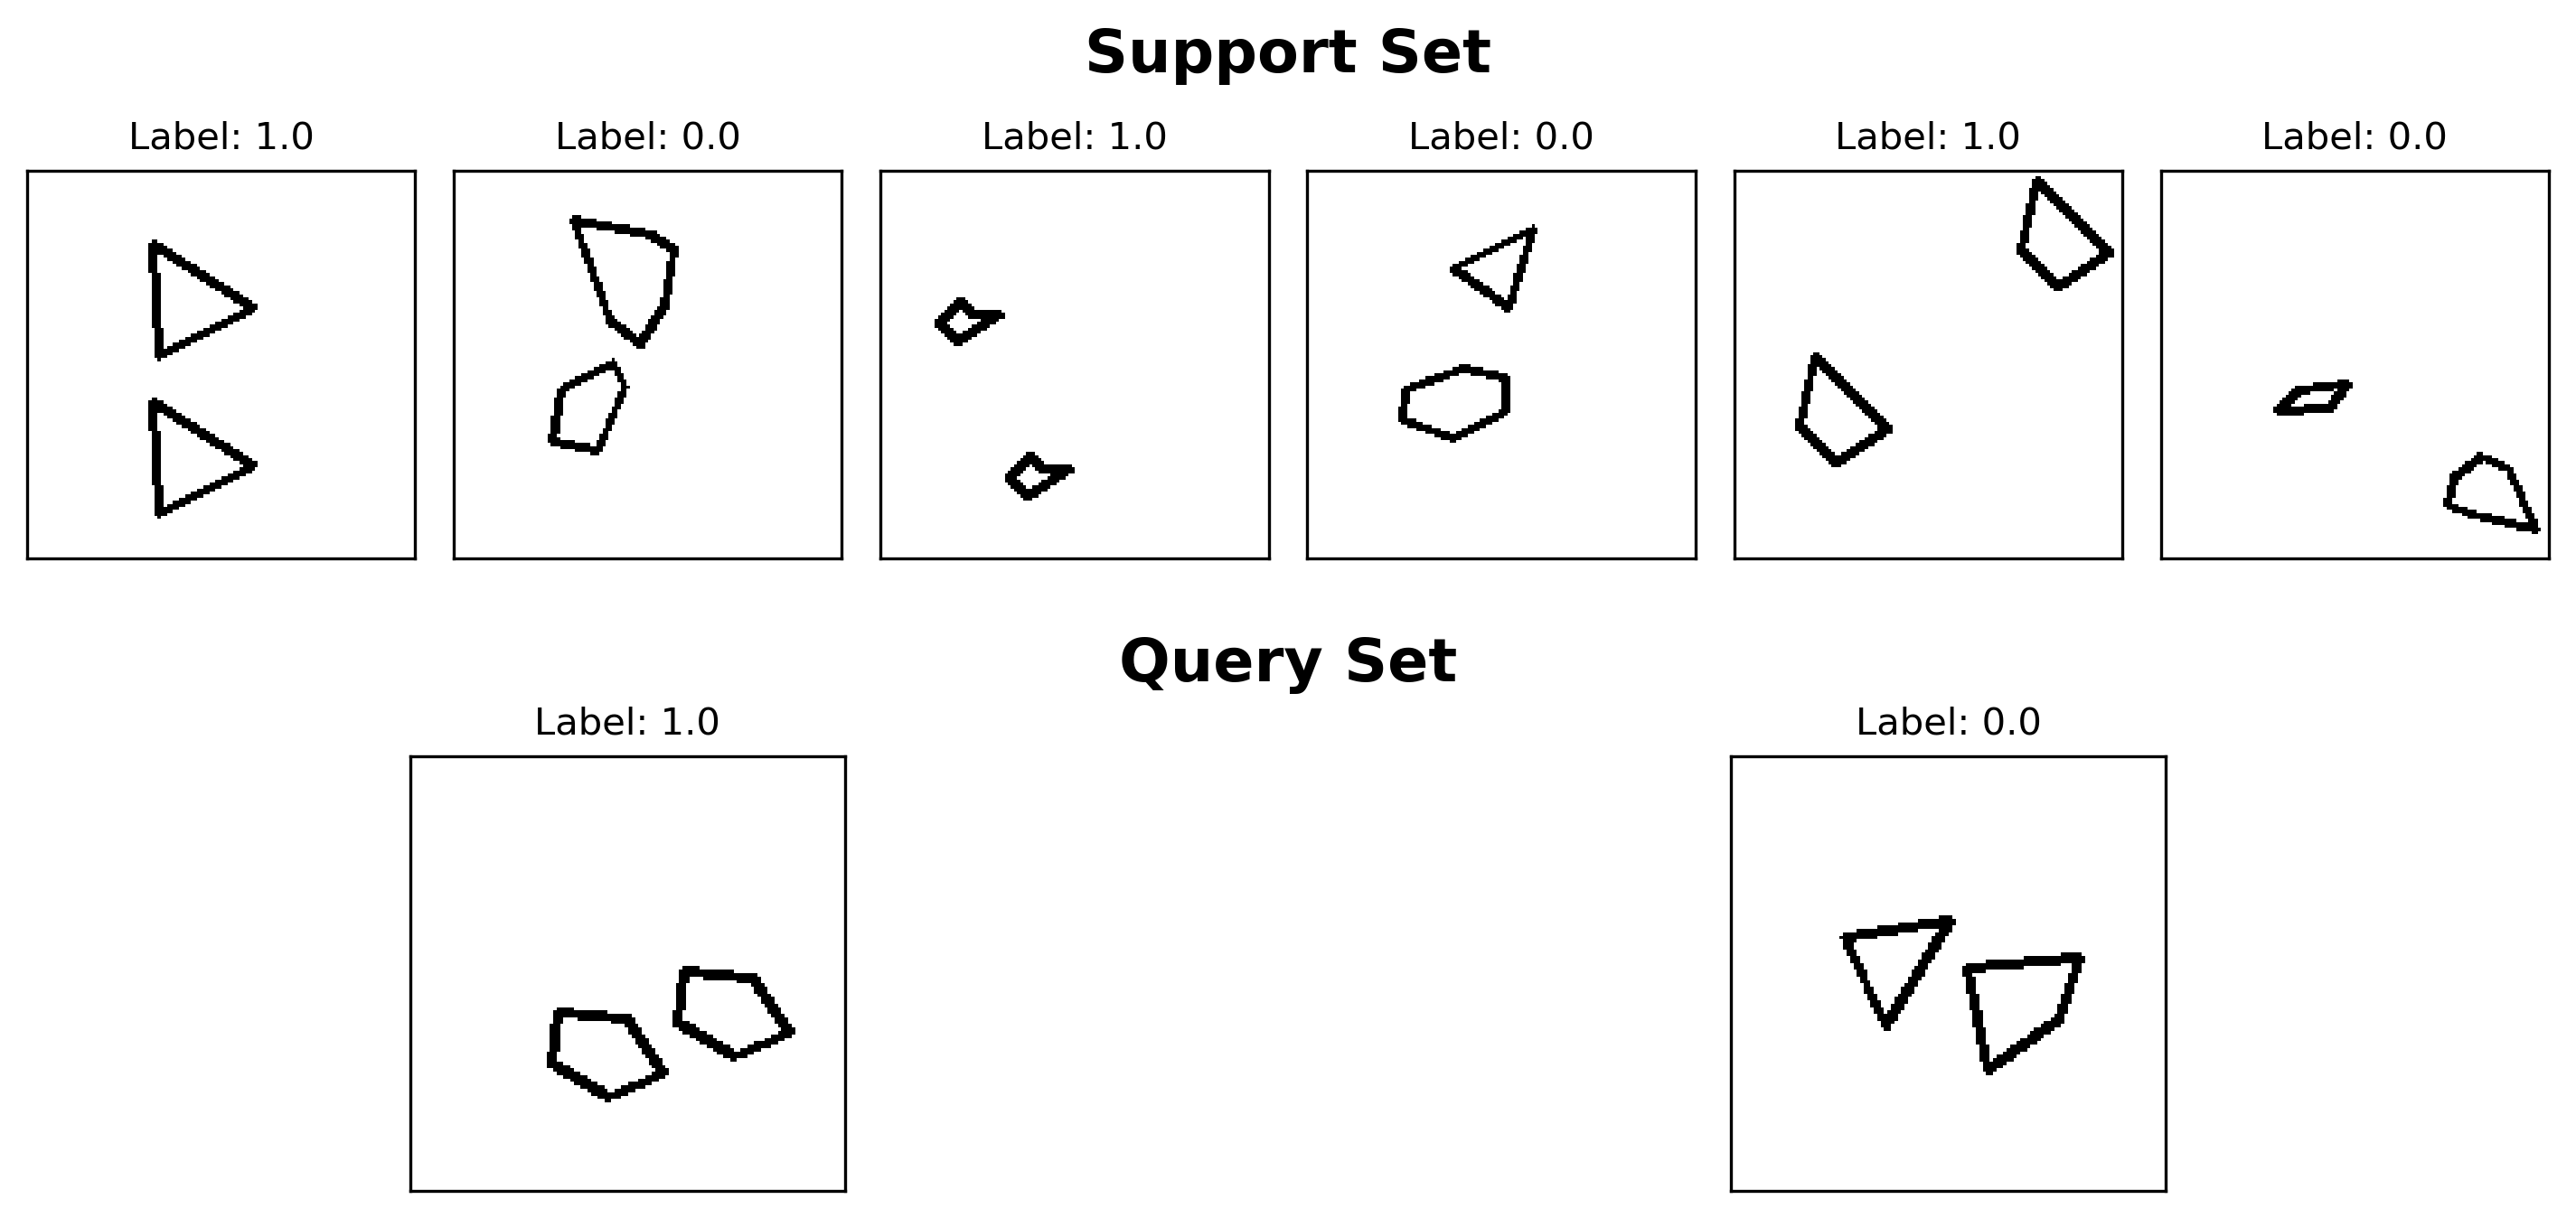
\includegraphics[width=0.9\columnwidth]{figures/wider_line_support6_ep0_boxed.png}
    \caption{An episode from the 'wider line' task with a support set of 6 examples.}
    \label{fig:wider_line_episode}
\end{figure}

\begin{figure}[H]
    \centering
    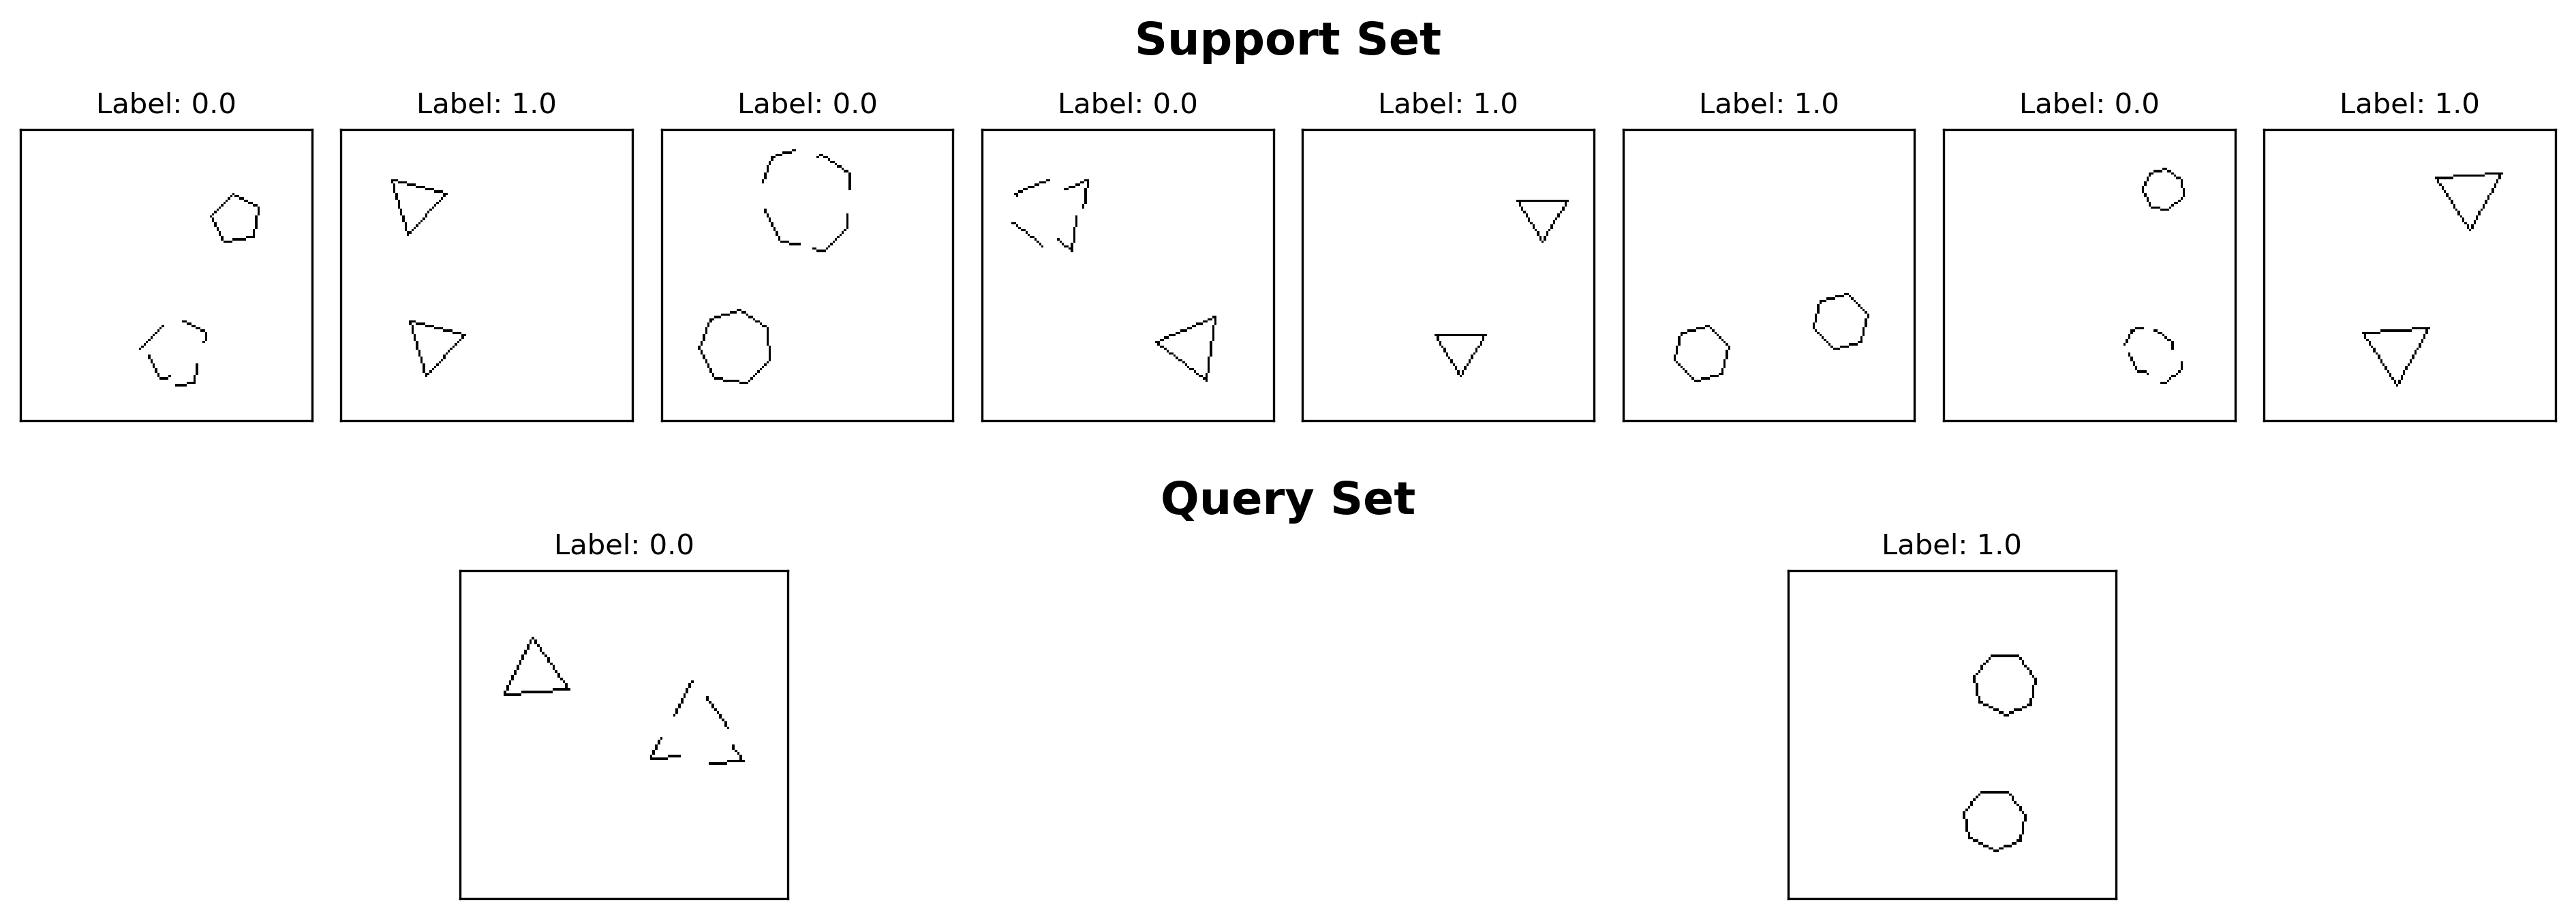
\includegraphics[width=0.9\columnwidth]{figures/scrambled_support8_ep0_boxed.png}
    \caption{An episode from the 'scrambled' task with a support set of 8 examples.}
    \label{fig:scrambled_episode}
\end{figure}

\begin{figure}[H]
    \centering
    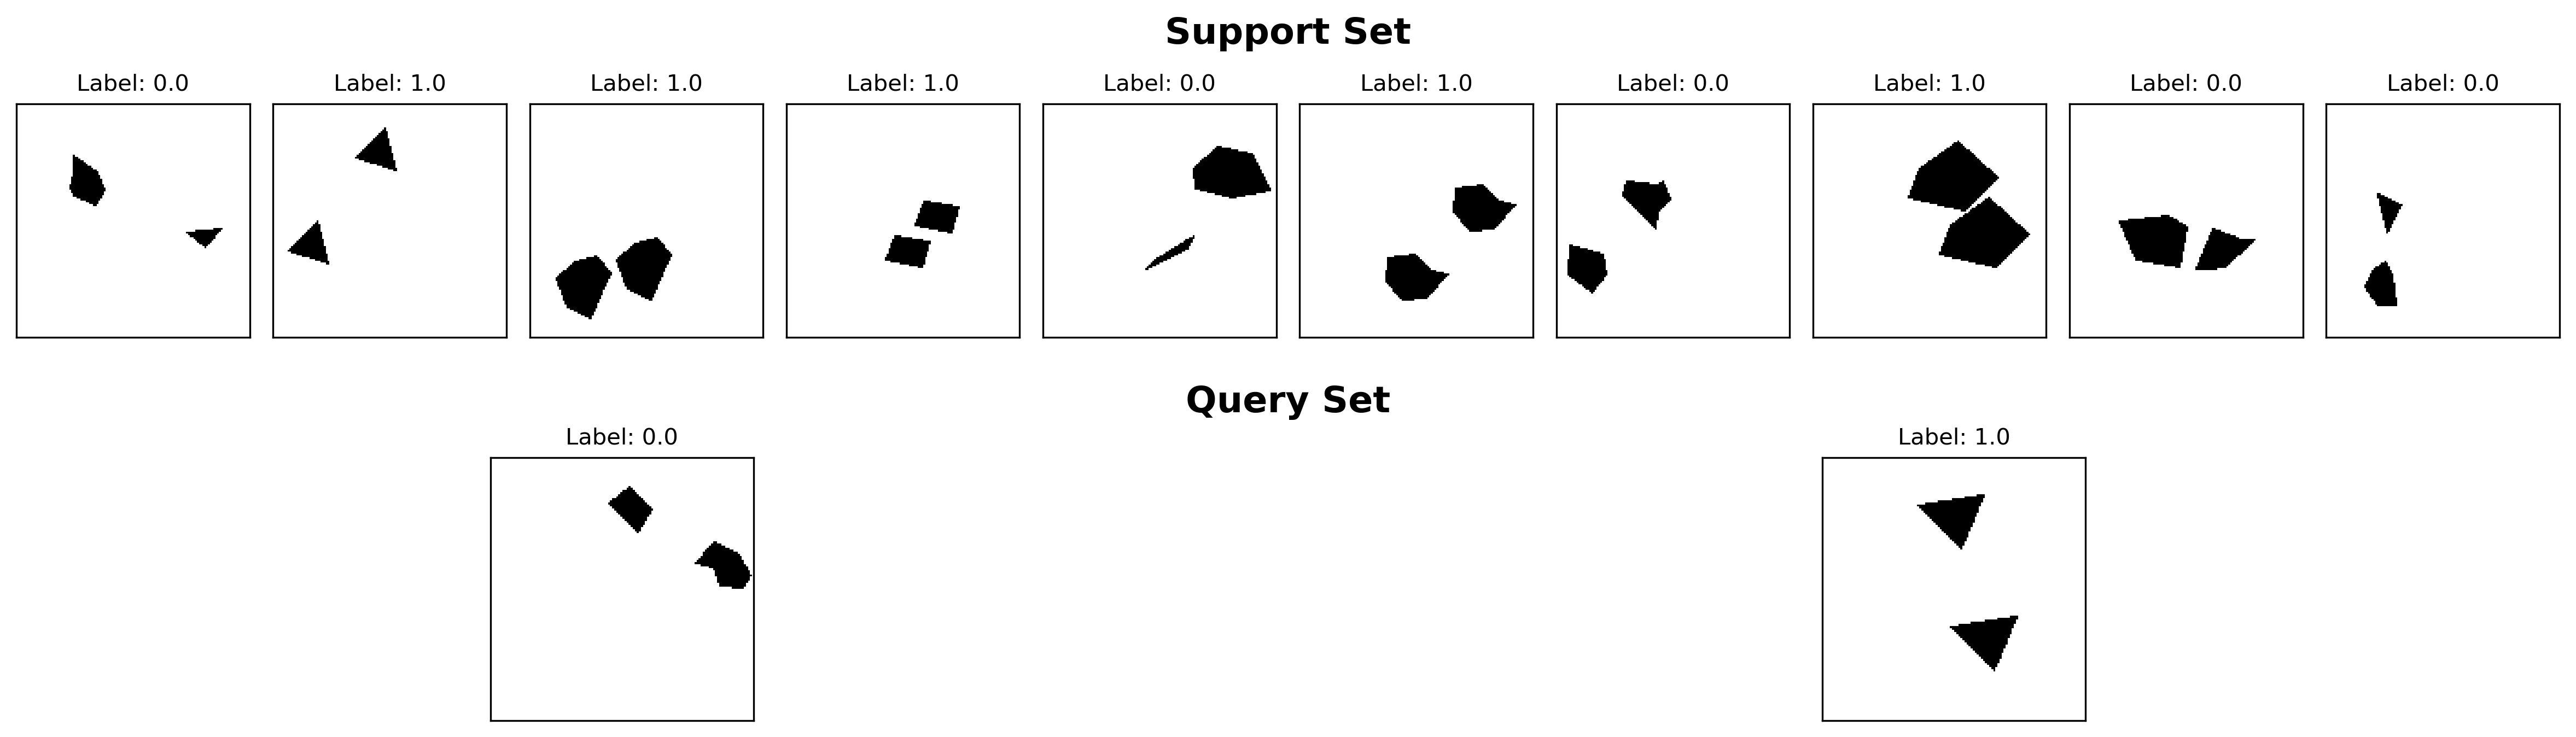
\includegraphics[width=0.9\columnwidth]{figures/filled_support10_ep0_boxed.png}
    \caption{An episode from the 'filled' task with a support set of 10 examples.}
    \label{fig:filled_episode}
\end{figure}

\end{document}
